\documentclass[12pt, a4paper]{article}

% --- Paquetes básicos ---
\usepackage[utf8]{inputenc}
\usepackage[spanish]{babel}
\usepackage[margin=2.5cm]{geometry}
\usepackage{graphicx}
\usepackage{float}
\usepackage{amsmath, amssymb}
\usepackage{fancyhdr}

% --- Configuración del Título ---
\title{Bloque 2: Simulación de Carga de Trabajo y Monitorización}
\author{Juan Reche Aguilar}
\date{\today}

% --- Configuración de Encabezados ---
\pagestyle{fancy}
\fancyhf{}
\rhead{Ingeniería de Servidores}
\lhead{Juan Reche Aguilar}
\cfoot{\thepage}

\begin{document}

\maketitle

\tableofcontents
\newpage

\section{Ejercicio 2.2.1 Carga Http con AB}

\begin{figure}[H]
    \centering

    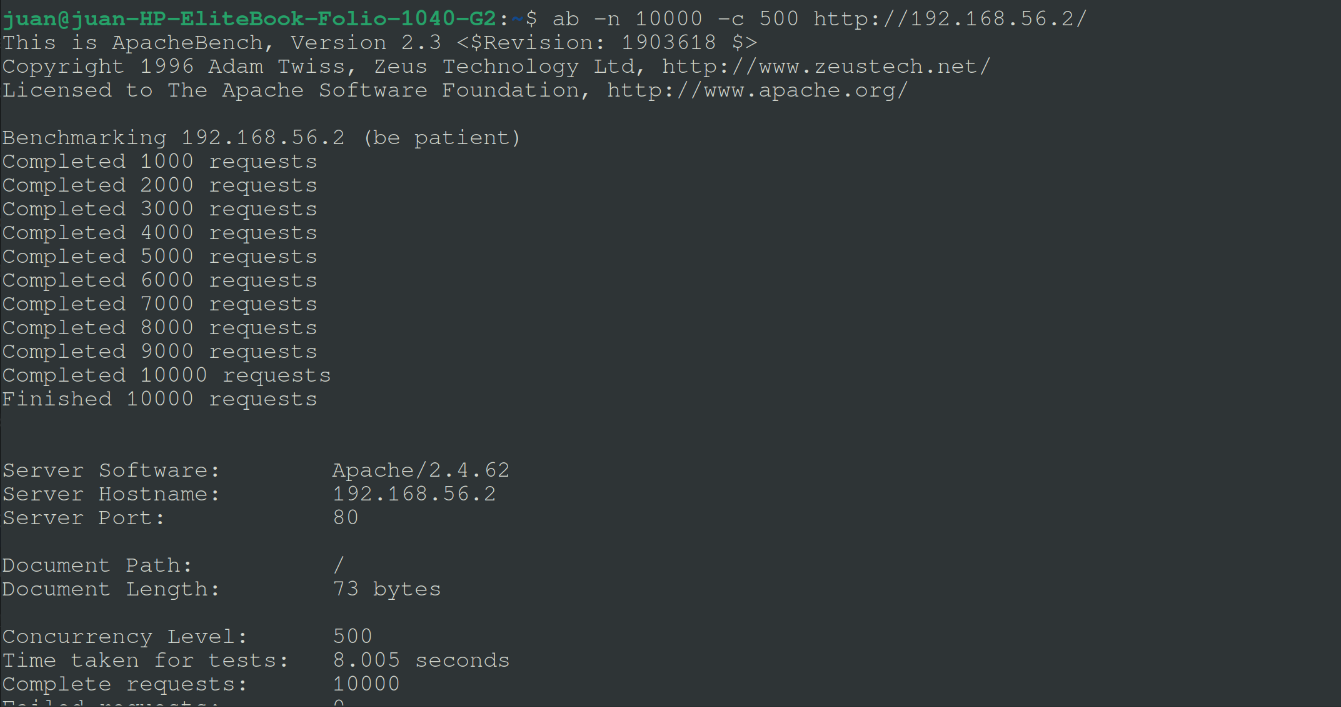
\includegraphics[width=1\textwidth]{../../capturas2/seccion2/apache1.png}

    \caption{Ejecucion sobre Apache\_1.}

    \label{fig:apache1}
\end{figure}

\begin{figure}[H]
    \centering

    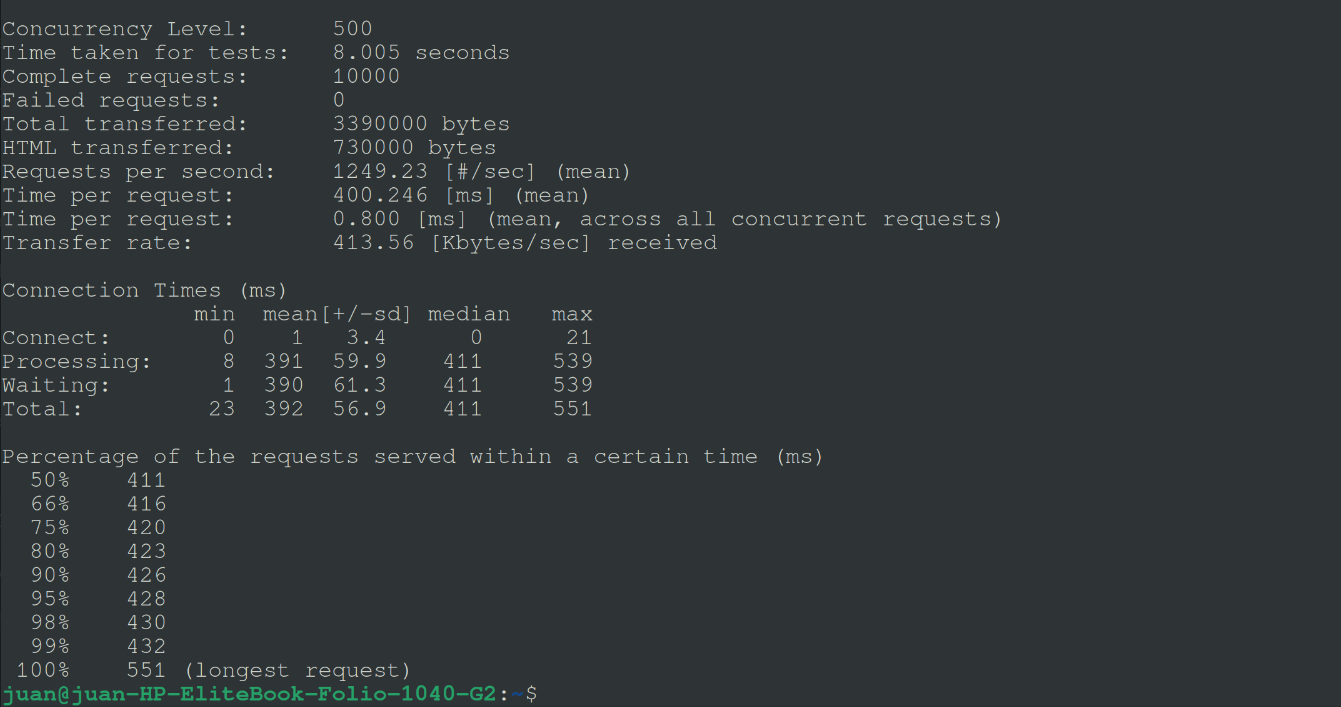
\includegraphics[width=1\textwidth]{../../capturas2/seccion2/apache2.png}

    \caption{Ejecucion sobre Apache\_2, continuación.}

    \label{fig:apache2}
\end{figure}

\begin{figure}[H]
    \centering

    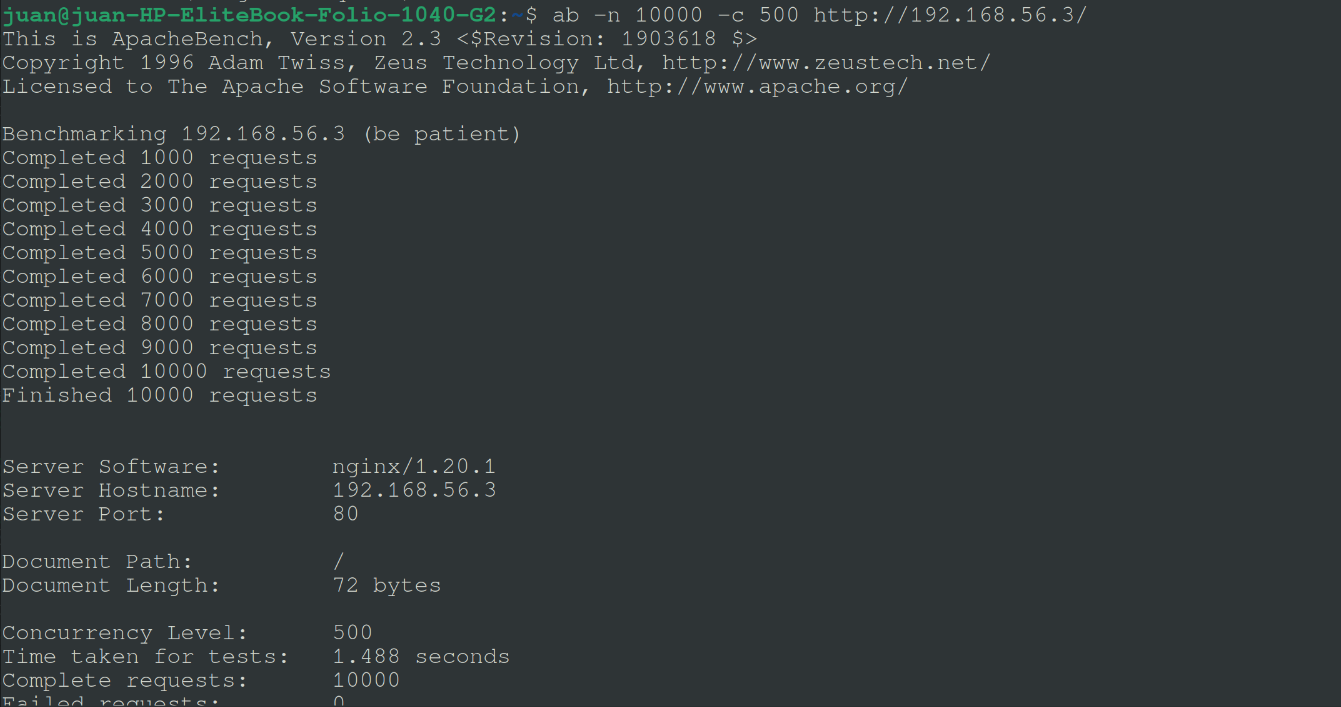
\includegraphics[width=1\textwidth]{../../capturas2/seccion2/nginx1.png}

    \caption{Ejecucion sobre Nginx\_1.}

    \label{fig:nginx1}
\end{figure}

\begin{figure}[H]
    \centering

    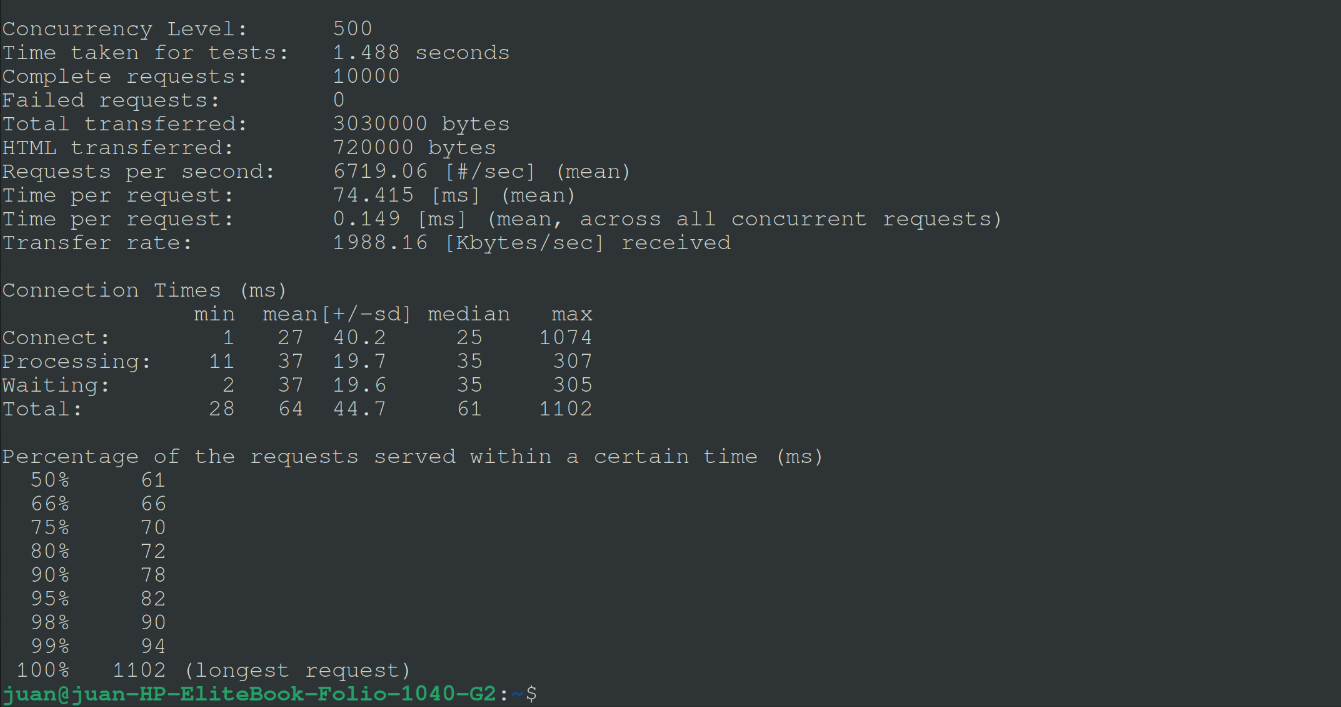
\includegraphics[width=1\textwidth]{../../capturas2/seccion2/nginx2.png}

    \caption{Ejecucion sobre Nginx\_2, continuación.}

    \label{fig:nginx2}
\end{figure}

En esta prueba de carga se ha empleado la herramienta Apache Benchmark (ab) para someter a los 
servidores web Apache y Nginx a un test de estrés idéntico. Se ha definido un entorno de ejecución exigente , 
lanzando un total de 10.000 peticiones con un nivel de concurrencia de 500 peticiones simultáneas 
sobre el archivo estático index.html por defecto. 
\\
Ambos servidores han demostrado una configuración robusta ante la carga exigida, 
logrando despachar la totalidad de la prueba sin registrar ninguna petición fallida (Failed requests: 0).
\\
Apache logró procesar una media de 1.249 peticiones por segundo (RPS), tardando aproximadamente 8 segundos en 
finalizar el test al completo. Su tiempo medio de respuesta por cada bloque de peticiones concurrentes fue de unos 
400 milisegundos.
\\
Nginx, por su parte, alcanzó una tasa de 6.719 peticiones por segundo (RPS), completando la misma carga en apenas 
1,48 segundos. El tiempo medio de respuesta cayó drásticamente a unos 74 milisegundos. 
Nginx demostró ser más de 5 veces más rápido procesando este volumen.
\\
Estas diferencias de rendimiento eran esperadas debido a la diferencia de arquitecturas entre ambos servidores.

\end{document}